\documentclass[border=8pt]{standalone}
\usepackage{tikz}
\usepackage{xcolor}
\usetikzlibrary{positioning,arrows.meta,shapes.geometric,calc}

\definecolor{obsCol}{HTML}{E66101}
\definecolor{genCol}{HTML}{5E3C99}
\definecolor{qCol}{HTML}{2166AC}
\definecolor{qualCol}{HTML}{B2182B}
\definecolor{quantCol}{HTML}{F4A582}
\definecolor{concCol}{HTML}{4DAF4A}
\definecolor{bgGray}{HTML}{F5F5F5}

\begin{document}
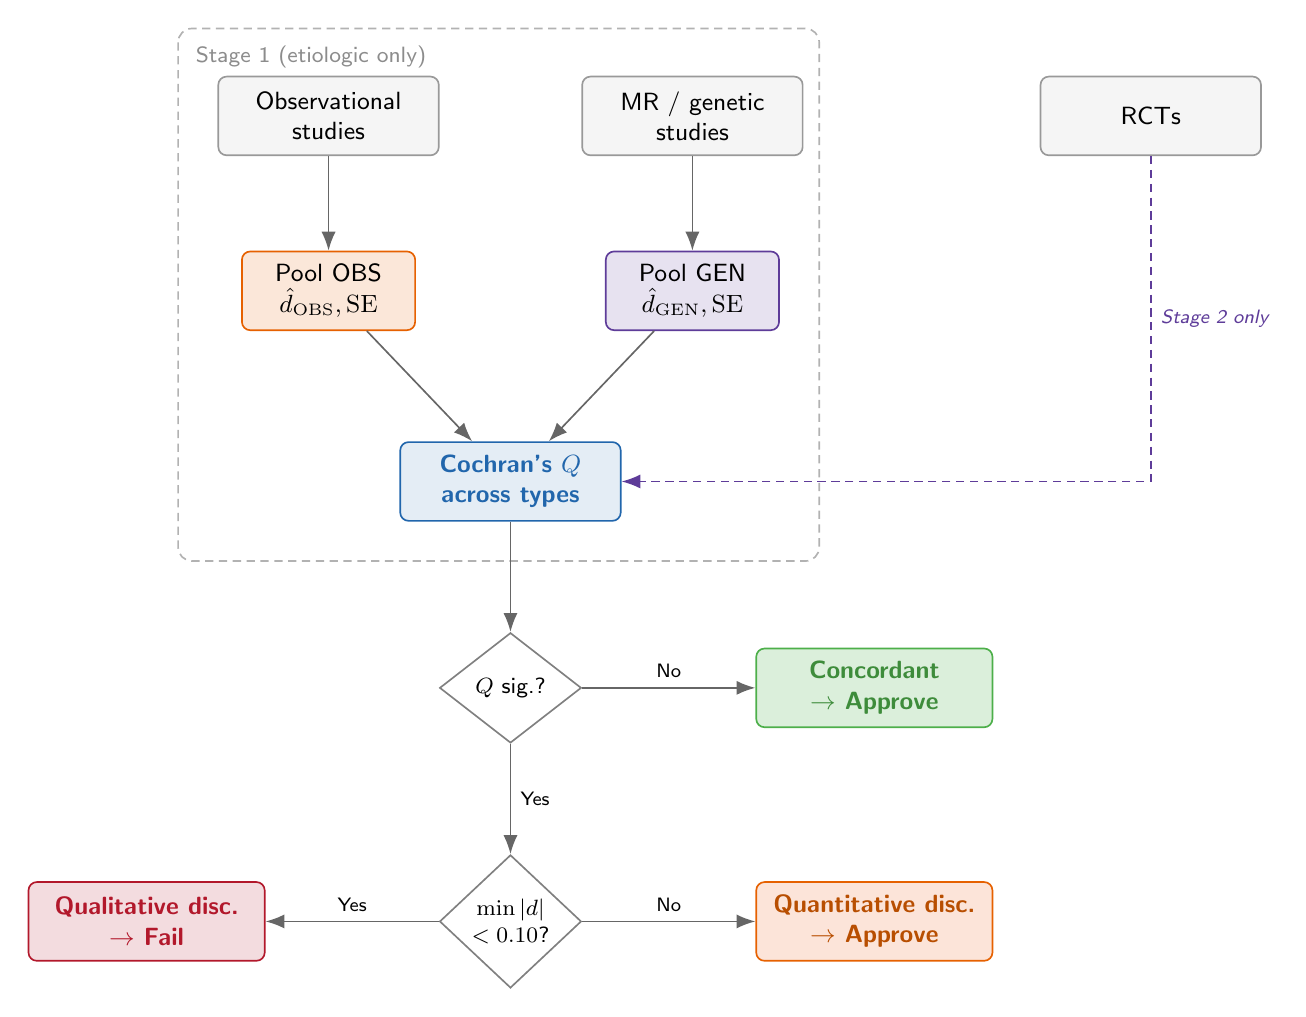
\begin{tikzpicture}[
    >={Latex[length=2.4mm,width=1.8mm]},
    font=\sffamily\small,
    node distance=10mm and 14mm,
    box/.style={rounded corners=3pt, draw, line width=0.6pt,
      minimum width=28mm, minimum height=10mm, align=center, inner sep=3pt},
    evidence/.style={box, fill=bgGray, draw=black!40},
    pool/.style={box, minimum width=22mm},
    test/.style={box, fill=qCol!12, draw=qCol, text=qCol, font=\sffamily\small\bfseries},
    outcome/.style={box, minimum width=30mm, font=\sffamily\small\bfseries},
    arr/.style={->, line width=0.6pt, draw=black!60},
  ]

% Evidence inputs
\node[evidence] (obs) {Observational\\studies};
\node[evidence, right=18mm of obs] (mr) {MR / genetic\\studies};
\node[evidence, right=30mm of mr] (rct) {RCTs};

% Pool within type
\node[pool, fill=obsCol!15, draw=obsCol, below=12mm of obs] (pobs) {Pool OBS\\$\hat{d}_{\mathrm{OBS}}, \mathrm{SE}$};
\node[pool, fill=genCol!15, draw=genCol, below=12mm of mr] (pgen) {Pool GEN\\$\hat{d}_{\mathrm{GEN}}, \mathrm{SE}$};

% Q test
\coordinate (mid) at ($(pobs.south)!0.5!(pgen.south)$);
\node[test, below=14mm of mid] (qtest) {Cochran's $Q$\\across types};

% Stage 1 bracket — encompasses evidence inputs, pools, AND Q test
\draw[densely dashed, black!30, line width=0.6pt, rounded corners=5pt]
  ($(obs.north west)+(-5mm,6mm)$) rectangle ($(qtest.south -| pgen.east)+(5mm,-5mm)$);
\node[font=\sffamily\footnotesize, text=black!45, anchor=north west]
  at ($(obs.north west)+(-4mm,5mm)$) {Stage 1 (etiologic only)};

% Decision diamond
\node[diamond, draw=black!50, fill=white, line width=0.6pt,
      minimum width=18mm, minimum height=14mm, inner sep=1pt,
      below=14mm of qtest, font=\sffamily\footnotesize, align=center] (dec) {$Q$ sig.?};

% Concordant branch
\node[outcome, fill=concCol!20, draw=concCol, text=concCol!80!black,
      right=22mm of dec] (conc) {Concordant\\$\to$ Approve};

% Second decision
\node[diamond, draw=black!50, fill=white, line width=0.6pt,
      minimum width=18mm, minimum height=14mm, inner sep=1pt,
      below=14mm of dec, font=\sffamily\footnotesize, align=center] (dec2) {$\min|d|$\\$< 0.10$?};

% Qualitative branch
\node[outcome, fill=qualCol!15, draw=qualCol, text=qualCol,
      left=22mm of dec2] (qual) {Qualitative disc.\\$\to$ Fail};

% Quantitative branch
\node[outcome, fill=quantCol!30, draw=obsCol, text=obsCol!80!black,
      right=22mm of dec2] (quant) {Quantitative disc.\\$\to$ Approve};

% Arrows — main flow
\draw[arr] (obs) -- (pobs);
\draw[arr] (mr) -- (pgen);
\draw[arr] (pobs) -- (qtest);
\draw[arr] (pgen) -- (qtest);
\draw[arr] (qtest) -- (dec);
\draw[arr] (dec) -- node[above, font=\sffamily\scriptsize] {No} (conc);
\draw[arr] (dec) -- node[right, font=\sffamily\scriptsize] {Yes} (dec2);
\draw[arr] (dec2) -- node[above, font=\sffamily\scriptsize] {Yes} (qual);
\draw[arr] (dec2) -- node[above, font=\sffamily\scriptsize] {No} (quant);

% RCT arrow — down to Q test level, then left into it
\draw[arr, densely dashed, genCol]
  (rct.south) -- (rct.south |- qtest.east)
  node[right, font=\sffamily\scriptsize\itshape, text=genCol, pos=0.5] {Stage 2 only}
  -- (qtest.east);

\end{tikzpicture}
\end{document}
